%!TEX root=../../thesis_rui_almeida.tex
\section{The Experiment}%
\label{sec:the_experiment}

As stated in this chapter's introductory notes, this thesis main body of
work revolves around two base assumptions, our hypothesis. The first
one, about the information capturing by the idealised system, was
addressed in lkjashdkjh~\todo{reference the correct subsection after
merging with the mac branch}. The second, more physical in nature, is
the subject matter of this section. Our hypothesis states that the light
absorption between points $A$ and $B$ (let's call it $A_{AB}$) should be
equal to the difference of the absorptions in $A$ and $B$. We can write
this, in a \emph{Lambertian} manner as in
Equation~\ref{eq:lambertian_hypothesis}.

\begin{equation}
    \label{eq:lambertian_hypothesis}
    I_B = I_A \cdot \exp \bigg[-AB \cdot \sum_i \sigma_{ABi} \cdot
    c_{ABi}\bigg]
\end{equation}

This is to say that the light intensity reaching point $B$ is given by
the intensity reaching $A$, exponentially decreased by the absorbers at
interval $AB$. The intensities at $A$ and $B$ are written as in
Equation~\ref{eq:intensityAtAAndB}.

\begin{equation}
    \begin{aligned}
        \label{eq:intensityAtAAndB}
        I_B = I_0 \cdot \exp \bigg[ -L_B \cdot \sum_i \sigma_{Bi} \cdot
        c_{Bi} \bigg]\\
        I_A = I_0 \cdot \exp \bigg[ -L_A \cdot \sum_i \sigma_{Ai} \cdot
        c_{Ai} \bigg]
    \end{aligned}
\end{equation}

If we join all this information in the same expression, the equation is
transformed into its final form, presented in
Equation~\ref{eq:hypothesis_final_form}.

\begin{equation}
    \small
    \label{eq:hypothesis_final_form}
    I_0 \cdot \exp \bigg[ -L_B \cdot \sum_i \sigma_{Bi} \cdot
            c_{Bi} \bigg] = I_0 \cdot \exp \bigg[ -L_A \cdot \sum_i \sigma_{Ai} \cdot
            c_{Ai} \bigg] \cdot \bigg[-AB \cdot \sum_i \sigma_{ABi} \cdot
            c_{ABi}\bigg]
\end{equation}

Equation~\ref{eq:hypothesis_final_form} can be greatly simplified: we
take the natural logarithm of both sides and we state that $\sum_i
\sigma_{Xi} \cdot c_{Xi} = S_i$. These operations result in the
simplified form of Equation~\ref{eq:final_form_simplified}.

\begin{equation}
    \label{eq:final_form_simplified}
    L_B \cdot S_B = L_A \cdot S_A + L_{AB} \cdot S_{AB}
\end{equation}

Now, $L_X \cdot S_X$ can be thought of as the wavelength dependent light
absorption in path $X$. In this case, the wavelength interval is always
the same. We can therefore conclude that, theoretically, our
hypothesis is valid: light absorption between points $A$ and $B$ can be
expressed in terms of the absorption on both these points and
corresponds to their difference.

Although mathematically this seems clear-cut, in the real world things
can become more problematic, since we have to deal with the
imperfections that characterise a real physical system. Noise,
instrumental limitations, adverse environmental effects, etc.. The
experiment we describe in the next few paragraphs aimed at determining
target trace gas concentration in a set analysis field. This field is
dimension-wise compatible with those that would be employed in the final
working system. The experiment geographic information is presented in
Figure~\ref{fig:experiment_map}.

\begin{figure}[htpb]
    \centering
    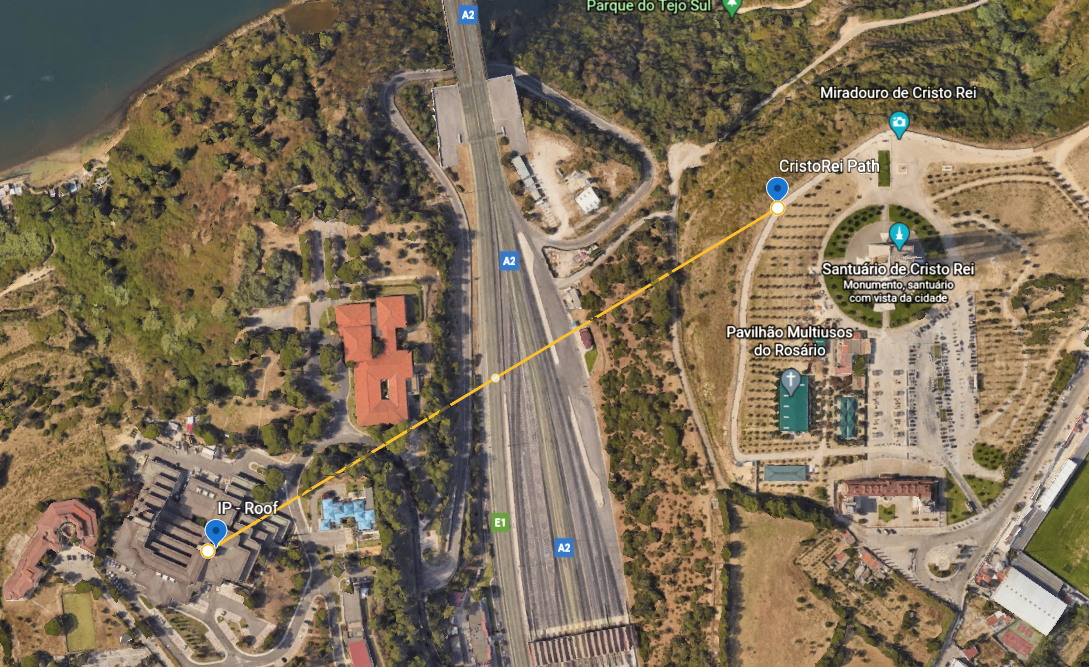
\includegraphics[width=0.8\linewidth]{img/png/experimentMap.png}
    \caption{Location of observer points for the physical experiment.}
    \label{fig:experiment_map}
\end{figure}
